\chapter{Methodology}

Our method uses a combination of different software both opened to university research purposes (MedInria) and developed in the lab for our very specific needs of reproducible experiments with comparable results \cite{piuzephd}. As explained in the previous section the first step is to use MedInria to read the DICOMs and get the tensor matrix \ref{diffusion_tensor_matrix} at every voxel, as well as the FA and ADC in reusable Matlab file format.

\section{Getting fiber directions from the diffusion tensor matrix}

Once we have our diffusion tensor matrix $\mathbb{D}$, a simple eigenvector and eigenvalue calculation gives us the eigenvalues $(\lambda_1, \lambda_2, \lambda_3)$ and the corresponding eigenvectors $(\nu_1, \nu_2, \nu_3)$.
\begin{align}
    \mathbb{D} &= \begin{pmatrix}
        D_{xx} & D_{xy} & D_{xz} \\
        D_{yx} & D_{yy} & D_{yz} \\
        D_{zx} & D_{zy} & D_{zz}
        \end{pmatrix} \\
    &= \mathbb{P}^{-1} \mathbb{\tilde{D}P}
\end{align}

where:

\begin{gather*}
    \mathbb{\tilde{D}} = \begin{pmatrix}
        \lambda_1 & 0 & 0 \\
        0 & \lambda_2 & 0 \\
        0 & 0 & \lambda_3
        \end{pmatrix} \\
    \mathbb{\tilde{D}}\cdot \nu_1 = \lambda_1 \nu_1 \\
    \mathbb{\tilde{D}}\cdot \nu_2 = \lambda_2 \nu_2 \\
    \mathbb{\tilde{D}}\cdot \nu_3 = \lambda_3 \nu_3
\end{gather*}
The biggest eigenvalue in absolute value will correspond to the fiber direction and sorting those will give us the eigenvector corresponding to the fiber direction. We can also at this point get the FA and ADC values to double check what MedInria gave us.

\section{Modeling fiber geometry using connection forms}

Connection forms measure the local rotations of the frame axes $\mathbf{f}_1, \mathbf{f}_2, \mathbf{f}_3$. Here we focus on the contraction of the 1-form $c_{1,2}$ on the frame axes $\mathbf{f}_3$ and compare its values in a short axis slice of a pig heart with an infarct \ref{fig:c123infarcted} with those in a short axis slice from a healthy pig heart \ref{fig:c123healthy}.
\begin{figure}[h!]
    \centering
    \begin{subfigure}[h!]{0.48\textwidth}
        \centering
        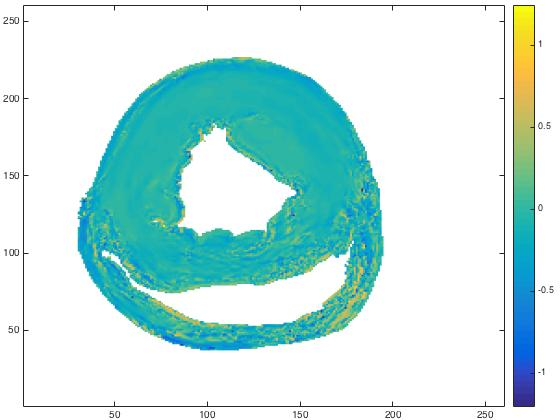
\includegraphics[width=\textwidth]{figures/pig4_c123_slice_19}
        \caption{$c_{1,2,3}$ (infarcted)}
        \label{fig:c123infarcted}
    \end{subfigure}
    \hfill
    \begin{subfigure}[h!]{0.48\textwidth}
        \centering
        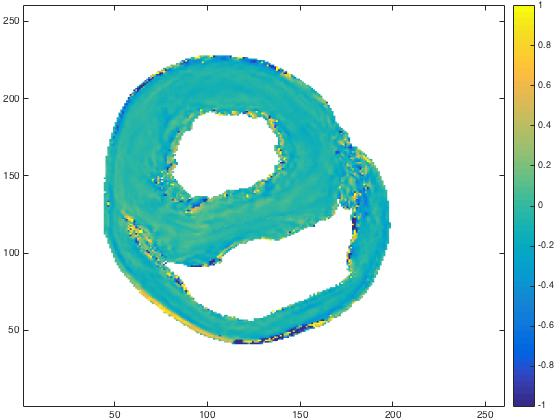
\includegraphics[width=\textwidth]{figures/pig25_c123_slice_30}
        \caption{$c_{1,2,3}$ (healthy)}
        \label{fig:c123healthy}
    \end{subfigure}
    \caption{$c_{1,2,3}$ with range of values in porcine hearts}
    \label{fig:c123all}
\end{figure}

On a qualitative approach, looking at the colors and comparing the smoothness of figures \ref{fig:c123infarcted} with the control health \ref{fig:c123healthy}, we can already notice how in the healthy case and in regions remote from the infarct in the infarcted case we have smooth and regular colors which represent a rather constant value of $c_{1,2,3}$. Whereas in the infarct region, it is clear that the values vary a lot more and give a strong impression of a lack of coherence.\\
A more quantitative approach will be discussed in Section \ref{histogram_section}.
 
 \begin{figure}
     \centering
     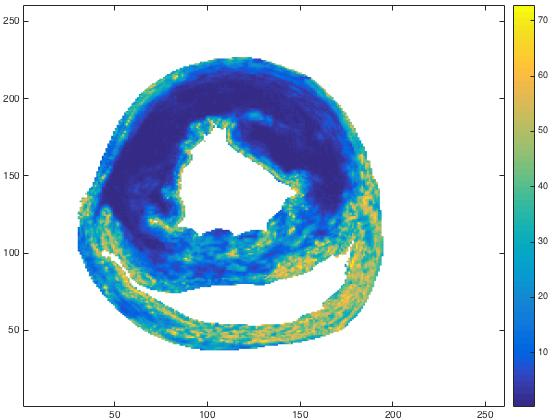
\includegraphics[width=\textwidth]{figures/pig4_error_of_fit_slice_19}
     \caption{Error of fit, giving the absolute angle difference between our estimation from the connection forms and the ground truth}
     \label{fig:error_of_fit}
 \end{figure}
 
Cartan frame field analysis applies to smoothly rotating frame fields. In the presence of infarcts fiber orientation coherence is lost. The connections then fail to explain the orientation of fibers in a local neighborhood and fitting errors using this method go up \ref{fig:error_of_fit}. This association of frame field fitting error with fiber incoherence is the key insight behind the developments in this thesis.

\section{Cartan Frame Fitting and Error Analysis}

As explained earlier, at each voxel we use an estimate of the fiber orientation given by the orientation of the first principal eigenvector of a diffusion tensor reconstruction for $\mathbf{f}_1$. We then estimate the heart wall normal as the gradient of the distance function to the boundary of the myocardium and take the component of the normal that is orthogonal to $\mathbf{f}_1$ to be $\mathbf{f}_3$. $\mathbf{f}_2$ is then taken to be their cross product. Our numerical implementation of frame field fitting relies on finding the best estimates of the 9 connection forms at each voxel in the sense of explaining the orientations in its neighborhood. Specifically, using Nelder-Mead optimization, we minimize an energy given by the angle between the measured orientation at each neighbor and that given by rotating the frame field by a particular set of connections \ref{fitting_method}. Once this method converges the error of fit at a voxel is taken to be the average angular error between fiber orientations in a neighborhood and those given by rotating the frame at that voxel using its connection parameters.